%!Mode:: "TeX:UTF-8"

\documentclass[19pt]{beamer}

\usepackage{xcolor}
\usepackage{soul}
\usepackage{url}

\setbeamertemplate{footline}[frame number]
\setbeamertemplate{navigation symbols}{}

\usetheme{Madrid}

\begin{document}

\title{The Design of BES DIRAC Transfer System}
\author{
    Zhang Xiaomei 
    \and
    Lin Tao 
}

\institute{IHEP}

\maketitle

\begin{frame}
    \frametitle{OUTLINE}
    \tableofcontents
\end{frame}

%\begin{frame}
% \frametitle{OUTLINE}
% \begin{itemize}
% \item
% \end{itemize}
%\end{frame}

\section{Purpose}

\begin{frame}
    \begin{center}
        \LARGE \tt{PURPOSE}
    \end{center}
\end{frame}

\begin{frame}
    \frametitle{Why we need a Transfer System?}
    \begin{block}{The basic functionalities}
        \begin{itemize}
            \item Transfer the production results to IHEP.
            \item Transfer {\tt DST} Files to sites.
        \end{itemize}
    \end{block}
    \begin{block}{What's more}
        \begin{itemize}
            \item When transfer the files in a dataset, users
                  don't need to always wait and monitor the results.
            \item If possible, the transfer system can try to re-transfer
                  the failed files.
            \item Administrators can monitor and analysis the status of the 
                  sites by the transfer monitor.
        \end{itemize}
    \end{block}
\end{frame}

\section{Requirements}

\begin{frame}
    \begin{center}
        \LARGE \tt{REQUIREMENTS}
    \end{center}
\end{frame}

\begin{frame}
    \frametitle{Requirements}
    \begin{block}{Users}
        \begin{itemize}
            \item Create datasets.
            \item Create dataset-based data transfer requests.
            \item Monitor the status of requests.
        \end{itemize}
    \end{block}
    \begin{block}{Administrators}
        \begin{itemize}
            \item Approve or Reject the requests.
            \item Check the health of transfer channels.
            \item View history of the transfer system.
        \end{itemize}
    \end{block}
\end{frame}

\section{Commands Design}

\begin{frame}
    \begin{center}
        \LARGE \tt{COMMANDs DESIGN}
    \end{center}
\end{frame}

\begin{frame}
    \frametitle{What are the Commands we may want}
    \begin{itemize}
        \item Create Transfer Request.
        \item List the detailed information of the request.
        \item List the status of the transfer system.
    \end{itemize}
    \begin{exampleblock}{Xiaomei's suggestion}
        \begin{itemize}
            \item {\tt BES-transfer-request-create datset dstSE}
            \item {\tt BES-transfer-request-list --requestID --user
                        --time\_create --status}
            \item {\tt BES-transfer-request-status requestID}
            \item {\tt BES-transfer-status}
        \end{itemize}
    \end{exampleblock}
\end{frame}

\begin{frame}
    \frametitle{the Commands already exists}
    \begin{description}
        \item[{\tt bes-dirac-dataset-create.py}]
            Create a Dataset with a list of {\tt LFN}.
        \item[{\tt bes-dirac-dataset-list.py}]
            List the {\tt LFN} in the dataset.
        \item[{\tt bes-dirac-transfer-create.py}]
            Create a transfer request with a dataset name.
        \item[{\tt bes-dirac-transfer-status.py}]
            Show the status of the Transfer Requests.
        \item[{\tt bes-dirac-transfer-show.py}]
            Show whole files associated with a special request.
    \end{description}
    \begin{block}{You can find the scripts in {\tt GitHub}}
        \url{https://github.com/mirguest/BESDIRAC/tree/master/TransferSystem/scripts}

        This system is still in evolutionary phase.
    \end{block}
\end{frame}

\section{Transfer System Design}

    %!Mode:: "TeX:UTF-8"
\begin{frame}
    \begin{center}
        \LARGE \tt{{\textsc{Transfer System Design}}}
    \end{center}
\end{frame}

\begin{frame}
    \frametitle{Introduction to the Transfer System}
    \begin{itemize}
        \item Our Transfer System is based on {\tt DIRAC}. %\footnote{http://diracgrid.org/}
        \item {\tt DIRAC} follows the {\tt Service Oriented Architecture (SOA)}
                paradigm, accompanied by a network of lightweight distribued
                agents which animate the system.
    \end{itemize}
    \begin{block}{DIRAC Architecture}
        \begin{columns}
            \column{.6\linewidth}
                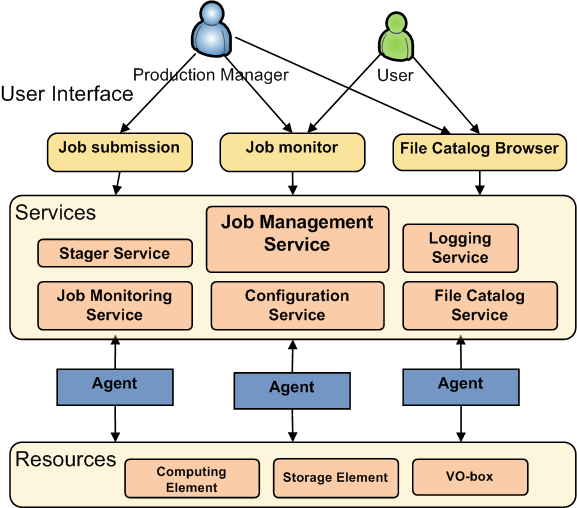
\includegraphics[height=5cm,keepaspectratio]{data/DIRAC_Architecture.png}
            \column{.4\linewidth}
                \begin{itemize}
                    \item User Interfaces
                    \item Services
                    \item Agents
                    \item Resources
                \end{itemize}
        \end{columns}
    \end{block}
\end{frame}

\begin{frame}
    \frametitle{Introduction to the Transfer System}
    \begin{itemize}
        \item In the transfer system, we have:
        \begin{itemize}
            \item {\tt Transfer Agent}.
            \item {\tt Transfer Request Service}.
            \item {\tt Dataset Service}.
        \end{itemize}
        \item {\tt Transfer Agent} is the scheduler to create the transfer 
              processes.
        \item {\tt Transfer Request Service} is to create and monitor the requests.
        \item The {\tt Transfer Agent} and the {\tt Transfer Request Service} 
              use database as their shared memory.
        \item {\tt Dataset Service} is to create a dataset. Because we don't have
              dataset support in DFC, we use this as a temporary solution.

    \end{itemize}
\end{frame}

\begin{frame}
    \frametitle{The Design of Transfer Agent}
    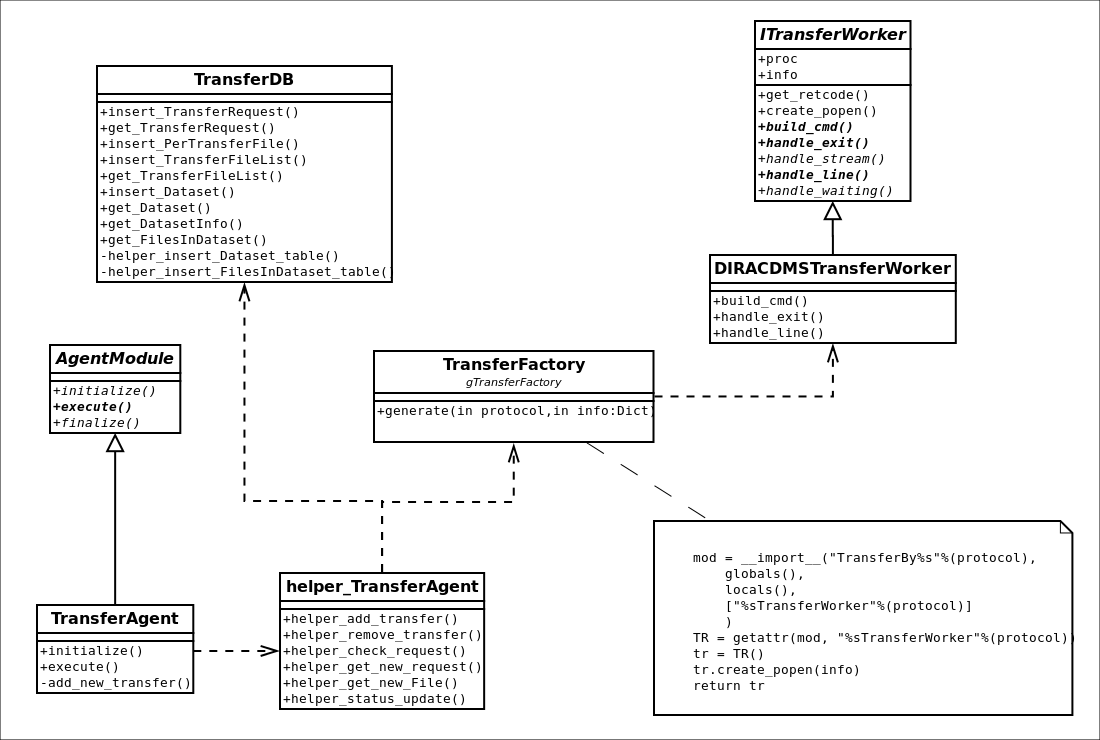
\includegraphics[height=8cm,keepaspectratio]{data/TransferAgent.png}
\end{frame}

\begin{frame}
    \frametitle{The Design of Transfer Agent}
    \begin{itemize}
        \item In {\tt DIRAC}, {\tt AgentModule} is the base class for all {\tt
            Agent}s. The derived classes can implement:
        \begin{itemize}
            \item {\tt initialize}
            \item {\tt execute}
            \item {\tt finalize}
        \end{itemize}
        \item {\tt TransferAgent} implements the {\tt non-blocking}
              scheduler in the {\tt execute} method.
        \item In fact, we create several {\tt sub processes} to run the 
                transfer commands. The scheduler uses the {\tt achychronous I/O}
                to communicate with the {\tt sub processes}.
        \item To test more easily, we create a standard module {\tt helper}.
              It just use the {\tt TransferDB} and some basic services supplied
              by {\tt DIRAC}, such as the {\tt Configuration Service}.
              So, we don't need to restart our agent to see what happens.
        \item To support multiple transfer protocols, we use a {\tt
                TransferFactory} to create {\tt TransferWorker}
    \end{itemize}
\end{frame}

\newsavebox{\TransferAgentExecute}
\begin{lrbox}{\TransferAgentExecute}
\begin{lstlisting}
def execute(self):
  # Handle the existed transfer worker
  for worker in self.transfer_worker[:]:
    retcode = worker.get_retcode()
    if retcode is not None:
      self.transfer_worker.remove(worker)
      # Handle retcode
      worker.handle_exit(retcode)
      self.helper.helper_remove_transfer(worker)
    else:
      worker.handle_waiting()
    pass
  else:
    pass
  # Create new transfer worker
  idle_worker = self.MAX_TRANSFER - len(self.transfer_worker)
  if idle_worker:
    for i in xrange(idle_worker):
      if not self.add_new_transfer():
        break
  return S_OK()
\end{lstlisting}
\end{lrbox}

\begin{frame}
    \frametitle{Implementation of the method {\tt execute}}
    \par\usebox{\TransferAgentExecute}
\end{frame}

\begin{frame}
    \frametitle{Implementation of the method {\tt execute}}
    \begin{itemize}
        \item The {\tt Transfer Worker} will manage the sub processes.
        \item We use the {\tt non-blocking I/O} to query 
              the status of the sub process.
        \item If the sub process exits, we can handle the exit 
              code by the {\tt Transfer Worker} itself.
        \item If the sub process is still running, we can 
              handle the output of the sub process.
        \item After check the workers, we create new workers
              to start the new transfer processes if there are
              idle slots.
        \item The status of the transfer requests are saved 
              in the {\tt MySQL} database.
    \end{itemize}
\end{frame}

\begin{frame}
    \frametitle{Table schemas}
    \begin{block}{Four tables in current database.}
    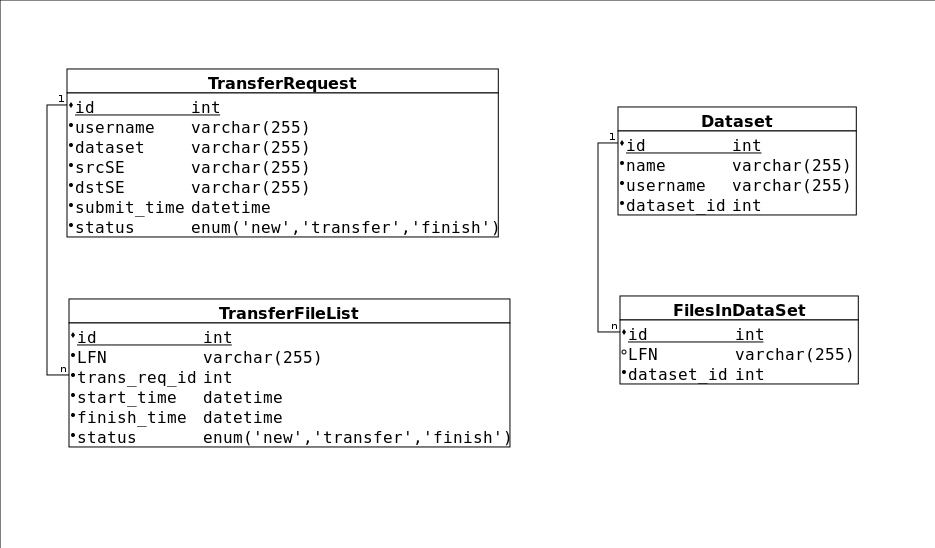
\includegraphics[width=12cm,keepaspectratio]{data/TransferDB.png}
    \end{block}
\end{frame}


\end{document}
